\chapter{\iflanguage{ngerman}{Übersicht Hybrider OP-Saal}{Overview}}
\label{sec:overview}

Weniger invasive Eingriffe, geringeres Risiko und kürzere Operations- und Krankenhausaufenthalte sind Anforderungen die heutzutage an Ärzte und Operationssäle gestellt werden \cite{DerDigitaleOperationssaal}. Diesen Anforderungen kann ein konventioneller OP-Saal nicht mehr gerecht werden. Aus diesem Grund findet ein Umstieg zum Hybriden/ Digitalen/ Multifunktionalen oder auch Hochpräzisions- OP-Saal statt. Dabei steht die Digitalisierung des OP-Saals und Integration Bildgebender Verfahren während der Operation im Vordergrund.

In den folgenden Kapiteln wird Hybrider OP-Saal als einheitliche Bezeichnung verwendet. Es werden die Unterschiede vom Hybriden zum Konventionellen OP-Saal herausgearbeitet, sowie Einsatzgebiete in welchen der Hybride OP-Saal seine Vorteile bringt.

\subsection{Hybrider OP-Saal vs. Konventioneller OP-Saal} 

\begin{figure} [H]
	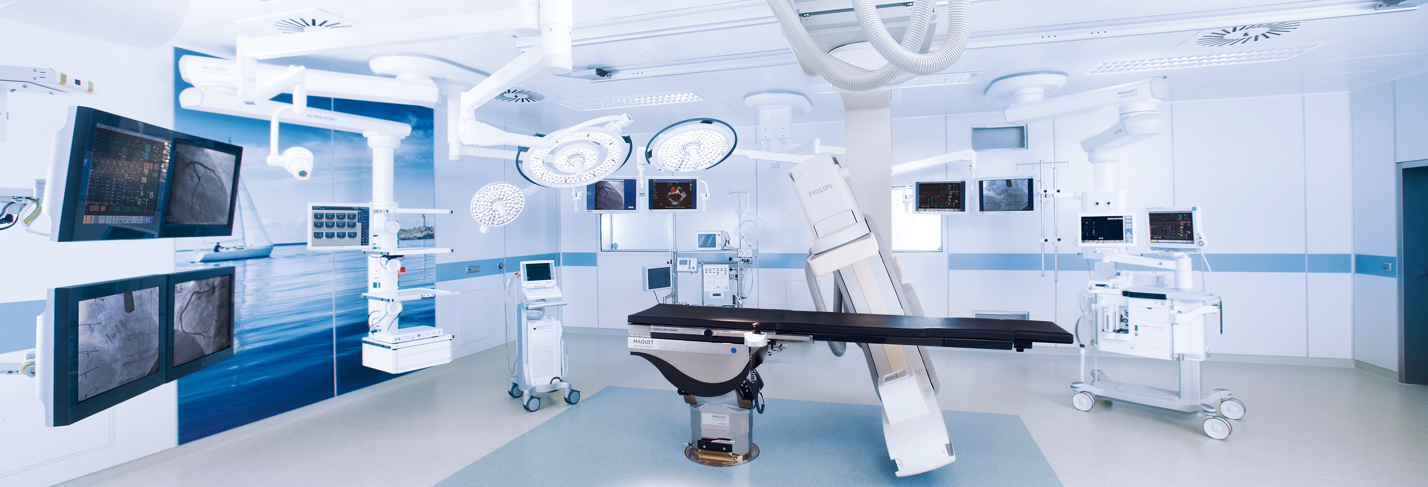
\includegraphics[scale = .3]{Content/Pictures/hybrid-or.png}
	\caption{Hybrider OP-Saal von Maquet mit einem an der Decke fixierten C-Bogen \cite{Maquet}.}
	\label{fig:hybridor}
\end{figure}

Ein Hybrider OP-Saal (Beispiel in Abb. \ref{fig:hybridor}) ist die Kombination aus einem sterilen konventionellen OP-Saal mit qualitativ hochwertiger Bildgebung. Hinzu kommen ein multifunktionaler OP-Tisch, digitale Datenregistrierung und Dokumentation sowie ungehinderter Datenaustausch innerhalb und außerhalb des OPs. Zur Steuerung und Kontrolle der Geräte und Systeme im OP-Saal steht eine zentrale Benutzeroberfläche zur Verfügung \cite{HybriderVsKonventioneller,KarlStorz}. Darüber hinaus ist ein Hybrider OP-Saal, gegenüber einem Konventionellen OP-Saal, ein fachbereichsübergreifender chirurgischer Arbeitsbereich. Er wird gleichermaßen von der Neurochirurgie, Gefäßchirurgie, Onkologie, Kardiologie, Unfallchirurgie und vielen weiteren Bereichen genutzt \cite{Getinge}.\\
Mobile C-Bogen sowie Ultraschall- und Endoskopiegeräte gehören zur Standardausrüstung in Konventionellen OP-Sälen \cite{TechnicalConsiderations}. Bei komplexen Operationsvorgängen wird jedoch leistungsstärkere Ausrüstung benötigt um beispielsweise die dünnen Führungsdrähte bei Transkathetertechniken zu visualisieren. Aus diesem Grund werden die mobilen C-Bogen durch befestigte ersetzt. Zur ergänzenden Ausrüstung des Hybriden OP-Saals können weitere Geräte für die intraoperative Bildgebung, wie Computertomographen (CT), Magnetresonanztomographen (MRT) oder Angiografieanlagen gehören \cite{OPderZukunft}. 
Die befestigten C-Bogen ermöglichen qualitativ hochwertige Echtzeitbildgebung mit Fluroskopie (Abb. \ref{fig:fluroscopy}) mit deren Hilfe Katheter durch den Körper geführt werden können. Ein weiteres Verfahren ist die Digitale Subtraktionsangiographie (Abb. \ref{fig:dsa}). Dabei werden zwei Bilder (mit und ohne Kontrastmittel) vom abzubildenden Gebiet angefertigt. Bei Subtraktion der beiden Bilder bleiben nur die Blutgefäße zurück \cite{CurrentAndFuture}. Darüber hinaus bieten MRT und CT die Möglichkeit hochauflösende Bilder von Geweben und Organen anzufertigen (Abb. \ref{fig:mrtct}).\\

\begin{figure}[!htb]
	\minipage{0.32\textwidth}
	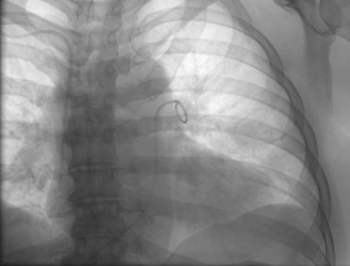
\includegraphics[width=\linewidth]{Content/Pictures/fluroscopy.png}
	\caption{Fluroskopie Aufnahme durch einen C-Bogen \cite{CurrentAndFuture}.}
	\label{fig:fluroscopy}
	\endminipage\hfill
	\minipage{0.32\textwidth}
	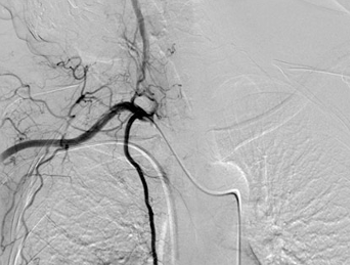
\includegraphics[width=\linewidth]{Content/Pictures/dsa.png}
	\caption{2D Bild mit Digitaler Subtraktionsangiographie (DSA) \cite{CurrentAndFuture}.}
	\label{fig:dsa}
	\endminipage\hfill
	\minipage{0.32\textwidth}%
	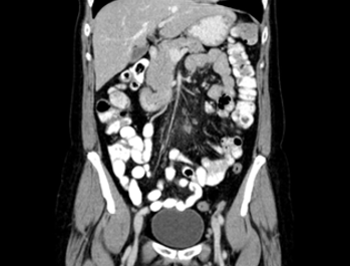
\includegraphics[width=\linewidth]{Content/Pictures/mrtct.png}
	\caption{CT-Aufnahme des Magens und Zwölffingerdarms \cite{CTBild}.}
	\label{fig:mrtct}
	\endminipage
\end{figure}

Somit können während eines Operationsvorgangs Diagnose und Therapiekontrolle vorgenommen, sowie minimal invasive Behandlungsverfahren durchgeführt werden \cite{SHG-Kliniken}. Ebenso ist es möglich \glqq während der Operation - und nicht erst danach - Bildkontrollen durch[zu]führen und allenfalls Korrekturmaßnahmen [zu] ergreifen\grqq{} \cite{OPderZukunft}. 

\subsection{Vorteile und wichtige Einsatzgebiete}

Wie Hybride OP-Säle Operationsvorgänge unterstützen, soll in der Neurochirurgie anhand der Kompensation des Brain Shifts, in der Gefäßchirurgie anhand des Setzens von Prothesen bei Aortenaneurysmen und in der Onkologie anhand der Tumorentfernung, erklärt werden.

\textbf{Neurochirurgie:}
Das Gehirn ist eine komplexe dreidimensionale Struktur, bei der sogenannte Brain Shifts (Verschiebungen der Gehirnstruktur Abb. \ref{fig:brainshift}) während einer Operation auftreten können. Ursachen für Brain Shifts können die Entfernung oder das Anschwellen von Gewebe, sowie der Verlust von Hirnwasser sein. Kommt es während einer Operation zu den genannten Verschiebungen, so stimmen die vor einer Operation angefertigten CT- oder MR-Bilder der Gehirnstruktur nicht mehr mit der aktuellen Struktur überein. Bild geführte neurochirurgische Systeme (Image Guided Neurosurgical Systems, kurz IGNS), die während der Operation als Navigationshilfe dienen, können wegen den inkorrekten Bilddaten nur begrenzt arbeiten \cite{BrainShiftInTumorResection}.\\
Intraoperativer Ultraschall (iUS) oder intraoperative MR-Bilder (iMR) können diesem Problem entgegenwirken und die fehlenden Informationen ergänzen, sodass IGNSs wieder einsetzbar sind. IMR ermöglicht während der Operation regelmäßig hochauflösende Bilder von der Gewebestruktur des Gehirns anzufertigen. Im Falle eines Brain Shifts kann entsprechend reagiert werden. Auch bei anderen neurochirurgischen Anwendungen wie der Hirnbiopsie, Entfernung von Tumoren oder der Drainage von Zysten kann iMR von Vorteil sein \cite{BrainShiftInTumorResection}.\\
Obwohl iMR als verlässlichste Option gilt, Bilder vom Gehirn anzufertigen und Brain Shifts zu erkennen, hat iUS den Vorteil kostengünstig Echtzeitzeitbilder zu produzieren. Die Kombination aus einem präoperativen MR-Bild und iUS reicht aus, um Gewebeveränderungen zu registrieren und die Korrektheit des IGNSs zu beurteilen. IMR hat eine Bildaufnahmezeit von 15 Minuten. Im Gegensatz dazu kann ein iUS Bild in 5 Minuten aufgenommen werden \cite{BrainShiftInTumorResection}. Aufgrund der vergleichbar schlechten Bildqualität gegenüber iMR wird iUS bisher begrenzt in der Neurochirurgie verwendet. Neue Ansätze (siehe Kapitel 4.1) ermöglichen jedoch die Möglichkeit einer genaueren US-Bildgebung für diesen Bereich \cite{BrainShiftInTumorResection}.

\begin{figure}[!htb]
	\minipage{0.45\textwidth}
	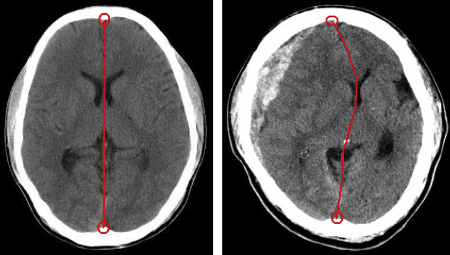
\includegraphics[width=\linewidth]{Content/Pictures/brainshift.png}
	\caption{(links) Keine Verschiebung, (rechts) Verschiebung der Mittellinie des Gehirns (midline brain shift) durch Anschwellen von Gewebe \cite{BrainShiftImage}.}
	\label{fig:brainshift}
	\endminipage\hfill
	\minipage{0.45\textwidth}%
	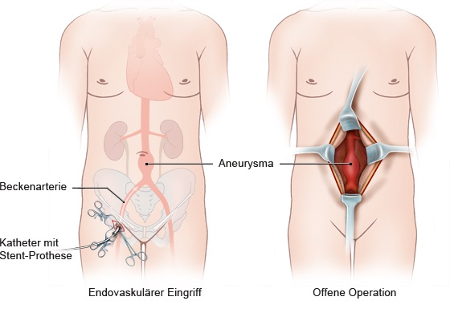
\includegraphics[width=\linewidth]{Content/Pictures/bauchaorten.png}
	\caption{(links) Endovaskulärer Eingriff bei einem Bauchaortenaneurysma mit Stent-Prothese gegenüber (rechts) einer offenen Operation mit normalen Prothesen \cite{BauaortenaneurysmaBild}.}
	\label{fig:bauchaorten}
	\endminipage
\end{figure}

\textbf{Gefäßchirurgie:}
Die Gefäßchirurgie profitiert von Hybriden OP-Sälen durch intraoperative Echtzeitbildgebung. Diese erlaubt den Fortschritt eines Katheters durch die Gefäße zu beobachten. Dadurch kann das Ergebnis, wie beispielsweise das richtige Sitzen einer Prothese, beurteilt werden \cite{DresdnerUniklinikum,TickendeBombeImBauch}. Für Aortenaneurysmen, krankhafte Erweiterungen der Hauptschlagader, ergeben sich alternative Möglichkeiten der Operationsdurchführung. Da Aortenaneurysmen ruptieren und zu lebensbedrohlichen Blutungen führen können, muss ab einem gewissen Durchmesser der Erweiterung eine Prothese gesetzt werden \cite{Aortenaneurysma}. Die Operation kann als offene Operation mit konventionellen Prothesen durchgeführt werden. Alternativ kann ein schonendes Verfahren mit Implantation großer maßgefertigter Gefäßprothesen im Hybriden OP-Saal (siehe Abb. \ref{fig:bauchaorten}) angewendet werden \cite{DresdnerUniklinikum}. \\
Bei offenen Operationen an Bauchaneurysmen muss ein großer Schnitt in die Bauchdecke gemacht werden. Trotz guter Langzeitergebnisse ist dieser Eingriff sehr belastend und mit vergleichsweise langen Erholungszeiten verbunden \cite{TickendeBombeImBauch}. Da Aortenaneurysmen verstärkt im höheren Alter (> 60 Jahre) auftreten, kommt für diese Patienten eine offene Operation nicht in Frage \cite{Aortenaneurysma}. \\
Alternativ wird deshalb beim schonenden Verfahren vor der Operation ein CT Bild angefertigt, welches mit den während der Operation entstehenden zwei- oder dreidimensionalen Bildern der Röntgenkontrolle kombiniert wird. Dies ermöglicht eine Stent-Prothese minimalinvasiv einzusetzen. Mithilfe eines Katheters kann dabei über einen kleinen Zugang in der Leiste durch das abgebildete Gefäß navigiert werden. Eine zusätzliche Software zur Navigationshilfe trägt dazu bei die Prothese durch die Gefäße ans Ziel zu bringen \cite{DresdnerUniklinikum,TickendeBombeImBauch}.

\textbf{Onkologie:}
In der Onkologie hat man im Hybriden OP-Saal den Vorteil, dass nach Entfernen eines Tumors vor Abschluss der Operation, ein MR-Bild gemacht werden kann. So kann sichergestellt werden, dass keine Rückstände des Tumors übersehen wurden, ohne den Patienten zu transportieren. Sollte das nicht der Fall sein, kann direkt nachkorrigiert werden. Durch diese Korrekturmöglichkeit können Folgeoperationen vermieden werden \cite{AerzteZeitung}. In mehr als einem drittel der Fälle, in denen die vollständige Entfernung eines Tumors angenommen wurde, sind mit iMR Rückstände festgestellt und nachkorrigiert worden \cite{BrainShiftInTumorResection}.

\textbf{Fazit:} Zusammenfassend ermöglichen Hybride OP-Säle präziseres, sicheres und schonenderes operieren durch minimalinvasive Eingriffe. Diese sind weniger belastend für den Patienten \cite{DresdnerUniklinikum}. Dies führt zu kürzeren Krankenhausaufenthalten und zu Kosteneinsparungen in der Nachbetreuung und -behandlung. Der beliebig positionierbare OP-Tisch in Kombination mit dem hochbeweglichen C-Bogen sorgen für bestmögliche Röntgenbildaufnahmen. Diese können zur Unterstützung vor, während und nach der Operation eingesetzt werden \cite{DresdnerUniklinikum}. Entscheidungen über den Fortlauf der Operation können so besser getroffen werden, Ergebnisse beurteilt und gegebenenfalls nachkorrigiert werden.

